\section{System Architecture}
\label{sec:system_architecture}

The system discussed in this chapter is a flight search engine in the form of a web application. This application should allow users to search for the best schedule, route and set of flights, for both one-way and round flights, as well as unconstrained multi-city trips. During the formal definition of the problem, in section \ref{sec:ftp}, it was shown that these problems can be converted into a Flying Tourist Problem instance, which is a generalization of the Traveling Salesman Problem. Because of this, as the number of cities increases, the problem becomes increasingly more difficult to solve. In order to cope with this, each user defined request is solved using the optimization algorithms previously  in chapter \ref{chap:os}.

The proposed system is fragmented into two separate applications, the Client Side (CSA) and the Server Side applications (SSA). The client side application is designed to solely interact with the user, redirecting  requests to the server side application, whose goal is to solve these requests. Thus, there is a complete separation of concerns between both applications: the CSA serves only as an input/output port, and the application logic and intelligence is handed by the SSA. The communication between both application relies on the Hypertext Transfer Protocol (HTTP) and on Asynchronous JavaScript and XML (AJAX). This means that the CSA may request data from the SSA using a simple HTTP protocol, and that this communication is asynchronous, allowing the user to continue to interact with the application, even while the response is being prepared. The structure of the proposed application, and the data-flow associated to the resolution of a user defined request, are presented in figure \ref{fig:sa_design}.

\begin{figure}[htpb]
  \centering
  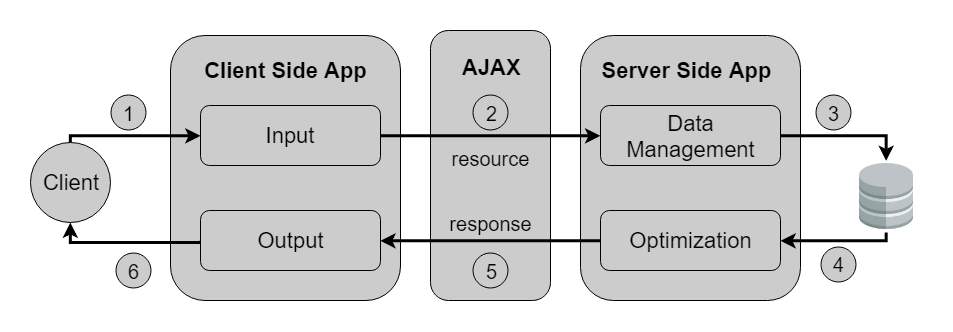
\includegraphics[width=\textwidth]{./Figures/system_design/system_architecture_design.png}
	\caption{Structure and data flow of the proposed application}
  \label{fig:sa_design}  
\end{figure}

